\documentclass{beamer}
\usetheme{Madrid}
\usecolortheme{default}


\usepackage[T1]{fontenc}
\usepackage[utf8]{inputenc}
\usepackage{amsmath,amssymb,bm,mathtools}
\usepackage{xcolor}
\usepackage{hyperref}
\usepackage{microtype}

\graphicspath{{./figures/}}
\usepackage{booktabs}


\title[Project 2]{Project 2}
\subtitle{CS 332, Fall 2025}
\author{Ben Cole \and Koshi Harashima}
\date{22 October, 2025}

\begin{document}

\maketitle

\begin{frame}{Outline}
  \tableofcontents
\end{frame}

%===================== we can skip this section! ==========================================
\section{Basic Setting}

\begin{frame}{Basic Setting : Online Learning}
    \textbf{Online Learning}: 
    \begin{itemize}
        \item k actions
        \item n rounds
        \item action $j$'s payoff in round i ; $v_j^i \in [0,h]$
        \item in round i:
        \begin{itemize}
            \item choose an action $j^i$
            \item learn payoffs $v_1^i, \dots, v_k^i$
            \item obtain payoff $v_j^i$
        \item Payoff $ALG = \sum_{i = 1} ^n v_j^i$
        \item the best in hindsight payoff is 
        \[
        OPT = max_j \sum_{i = 1} ^n v_j^i
        \]
        \item the regret of the algorithm is 
        \[
        Regret_n = \frac{1}{n}[OPT - ALG]
        \]
        \end{itemize}   
    \end{itemize}
\end{frame}

\begin{frame}{Basic Setting : EW Algorithm}
    \textbf{Algorithm}\\
    Exponential Weight Algorithm is implemented as follow; 
    \begin{itemize}
        \item learning rate $\epsilon$
        \item let $V_j^i = \sum_{r = 1}^i v_j^i$
        \item in round i choose j with probability $\pi_j^i$ proportional to $(1+\epsilon)^{\frac{V_j^{i-1}}{h}}$
        \item implemented as follow;
        {\small
        \[
            \pi_j^i = \frac{(1+\epsilon)^{\frac{V_j^{i-1}}{h}}}{\sum_{j'}(1+\epsilon)^{\frac{V_{j'}^{i-1}}{h}}}
        \]}
    \end{itemize}
    \textbf{learning rates}\\
    \begin{itemize}
      \item No learning: \(\epsilon = 0\) .
      \item Theoretical: \(\epsilon = \sqrt{\ln k / n}\).
      \item FTL:  \(\epsilon \approx \infty\).
    \end{itemize}
\end{frame}

\begin{frame}{Basic Setting; MC Simulation}
    we implemented MC Simulation as follow;
    \begin{itemize}
        \item fix k, n
        \item for each times, 
        \begin{enumerate}
            \item set $\epsilon$ to {$0.0001, \sqrt{log\frac{k}{n}}, 10000$}
            \item simulate it through implemented algorithms in each setting.
            \item calculate Regret (total Payoff, and his set of choices)
        \end{enumerate}
        \item then aggregate these results, and calculate mean of Regret and their confident intervals.
    \end{itemize}
\end{frame}
%===================== we can skip this section! ==========================================

\section{Part1}
\begin{frame}{Part1}

In Part 1, we consider two things;
\begin{enumerate}
    \item Adversarial Fair Payoffs (AFP) 
    \item Bernoulli Payoffs (BP)
\end{enumerate}
\end{frame}

\subsection{A: AFP}
\begin{frame}{A- Adversarial Fair Payoffs:}
       In each round i:
    \begin{itemize}
        \item Draw a payoff $x \sim U[0,1]$ (i.e., from the uniform distribution on interval [0,1])
        \item Assign this payoff to the action $j^*$ that has the smallest total payoff so far,\\
        i.e., $j^* = \arg\min_j V^{i-1}_{j} \quad \text{where} \quad V^{i}_{j} = \sum_{r=1}^{i} v^{r}_{j}$
        \item (All other actions get 0 payoff in round i.)
    \end{itemize} 
\end{frame}

\begin{frame}{A - Results}
    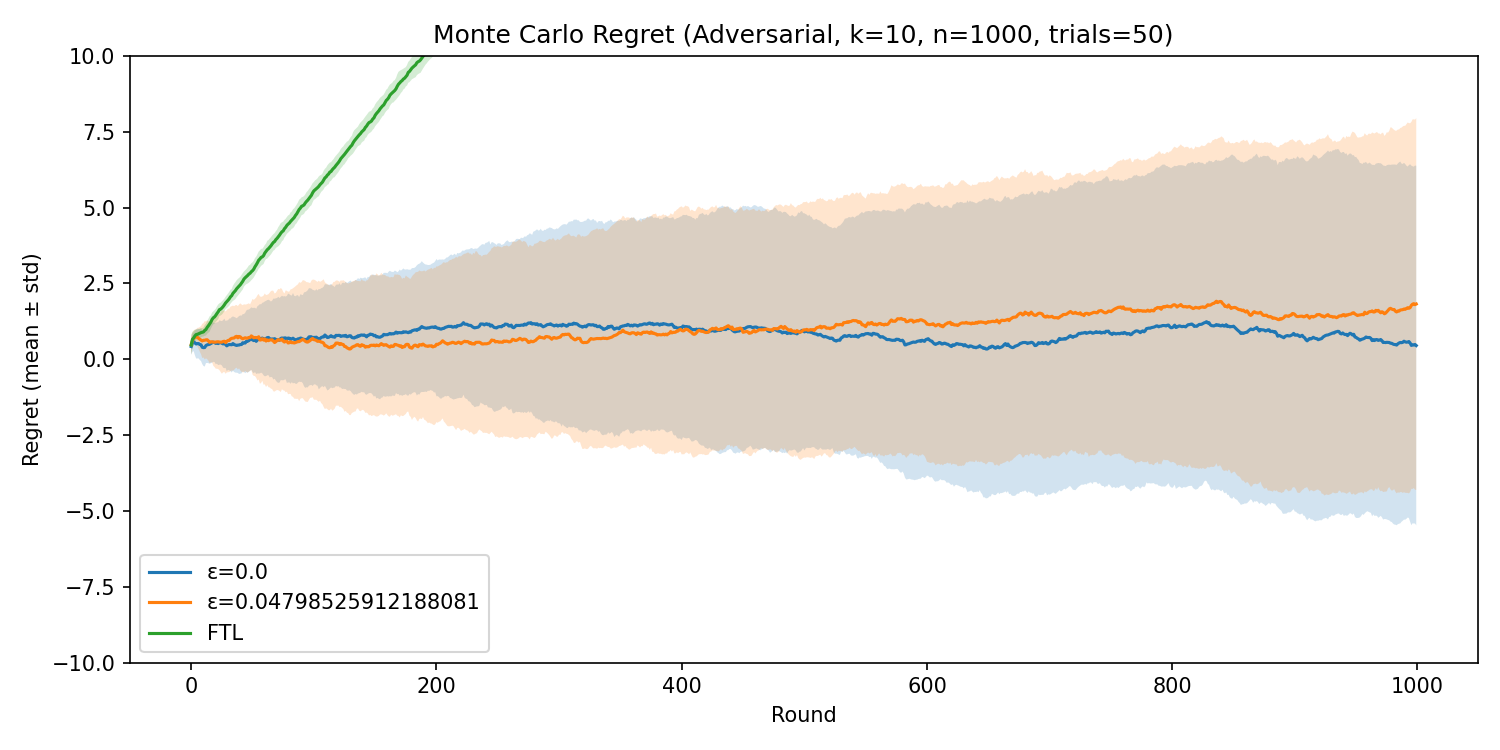
\includegraphics[width=0.9\textwidth]{figures/adv_mc_regret.png}
    we concluded that this results is consistent with the intuition that more you want to win profit, the less profit you win because of the fair structure of this game.
\end{frame}

\subsection{B : BP}

\begin{frame}{B - Bernoulli Payoffs:}
    Fix a probability for each action $p_{1},...,p_{k}$ with each $p_{k}$ in [0,1/2].\\
    In each round i,
    \begin{itemize}
        \item draw the payoff of each action j as $v^{i}_{j} \sim B(p_{j})$ (i.e, from the Bernoulli distribution with probability $p_j$ of being 1 and probability $1-p_{j}$ of being 0).
    \end{itemize}
\end{frame}

\begin{frame}{B - Results}
    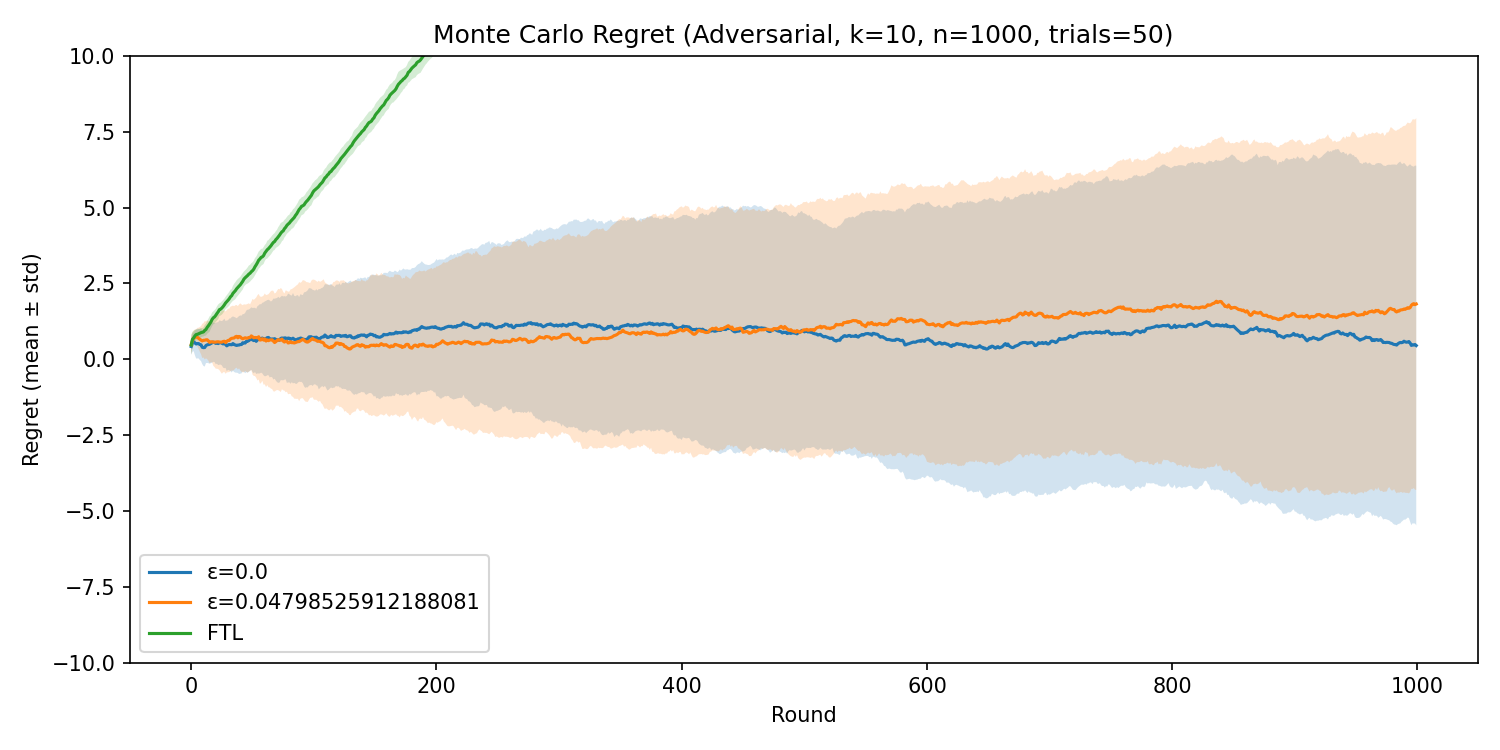
\includegraphics[width=0.9\textwidth]{figures/adv_mc_regret.png}
    we concluded that this results is consistent with the intuition that 
\end{frame}


\section{Part2}

\begin{frame}{Part2}
In Part 2, we consider two things;
\begin{enumerate}
    \item EW algorithm applied to Pachinko Payoffs (PP)
    \begin{itemize}
        \item This is very close setting as Multi-Bandit Problem.
    \end{itemize}
    \item Research Payoffs (RP)
    \begin{itemize}
        \item we modeled our research environment; characterizing research style with AI.
    \end{itemize}
\end{enumerate}
    
\end{frame}

\subsection{C : PP}

\begin{frame}{C}
In this part, we collect data from Japanese Pachinko (slot machine in Japan).\\
Here's our setting. Simple model with state transition model.
\begin{itemize}
    \item There are two conditions(unobservable)
    \begin{itemize}
        \item Normal condition
        \item Rush condition
    \end{itemize}
    \item In each setting, the chance of winning or losing is assigned.
\end{itemize}
\begin{itemize}
    \item we collect folloing data; 
    \begin{itemize}
        \item 1. payoff
        \item 2. probability of winning for each state.
        \item 3. probability of condition transition for each state.
    \end{itemize}
    \item there's five famous machines whose payoffs and probabilities differ from each other.
\end{itemize}
\end{frame}

\begin{frame}{C - Description of Machines}
5 machines; Tokyo Gouhl, Gundam Unicorn, Madoka Magica, Evangelion, Re.ZERO.
\begin{itemize}
    \item 1. Tokyo Gouhl
    \begin{itemize}
        \item low probability of winning, highest profit
    \end{itemize}
    \item 2. Gundam Unicorn
    \begin{itemize}
        \item middle
    \end{itemize}
    \item 3. Madoka Magica 
    \begin{itemize}
        \item middle
    \end{itemize}
    \item 4. Evangelion
    \begin{itemize}
        \item In rush state, profit is insane.
    \end{itemize}
    \item 5. Re.ZERO
    \begin{itemize}
        \item high average performance
    \end{itemize}
\end{itemize}
\end{frame}

\begin{frame}{C - Results}

    
\end{frame}


\begin{frame}{C - Image}
    
\end{frame}

\begin{frame}{C - Graghs}

    
\end{frame}



\subsection{D : RP}
\begin{frame}{D -}
    
\end{frame}

\begin{frame}{D - Results}

    
\end{frame}

\section{Usage of AI}
\begin{frame}{Usage of AI}
    AI was used for coding; final review and responsibility by the authors.
\end{frame}

\end{document}